\documentclass[times, 10pt,twocolumn]{article}
\usepackage{latex8}
\usepackage{times}

\usepackage{amssymb}
\usepackage{amsfonts}
\usepackage{amsmath}
\usepackage{verbatim}
\usepackage{graphicx}

\newcommand{\Y}[2]{{\cal Y}^{#1}_{#2}}
\newcommand{\Prob}[3]{{\cal P}_{#1 #2}(#3)}

\pagestyle{empty}

\begin{document}

\bibliographystyle{abbrv}

\title{A Markov Reward Model Checker}
\author{
   Joost-Pieter Katoen{$^{\ddagger,\dagger}$},
   Maneesh Khattri{$^{\dagger}$}
   and Ivan S.\ Zapreev{$^{\dagger}$}
   \and
   {$^{\dagger}$}
   \small{University of Twente, P.O. Box 217, 7500 AE Enschede, 
           The Netherlands}\\
   \and
   {$^{\ddagger}$}\small{RWTH Aachen, Ahornstra\ss e 55, D-52072 Aachen, 
           Germany}
}

\maketitle
\thispagestyle{empty}

\begin{abstract}
This short tool paper introduces MRMC, a model checker for discrete-time
and continuous-time Markov reward models.
It supports reward extensions of PCTL and CSL, and allows for the automated
verification of properties concerning long-run and instantaneous rewards
as well as cumulative rewards.
In particular, it supports to check the reachability of a set of goal 
states (by only visiting legal states before) under a time and an accumulated 
reward constraint. 
Several numerical algorithms and extensions thereof are included in MRMC.
\end{abstract}


%------------------------------------------------------------------------- 
\Section{Introduction}

Model checking is an automated technique that establishes whether certain 
qualitative properties such as deadlock-freedom or request-response 
requirements (``does a request always lead to a response?'') hold in a
model of the system under consideration.
Such models are typically transition systems that specify how the system
may evolve during execution.
Properties are usually expressed in temporal extensions of propositional
logic, such as CTL.

Since the seminal work of Hansson and Jonsson, adapting model checking to 
probabilistic systems has been a rather active research field.
This has resulted in efficient algorithms for model-checking DTMCs and 
CTMCs, as well as Markov decision processes, that are supported by several
tools nowadays such as ETMCC, PRISM, GreatSPN, VESPA, Ymer, and the APNN
Toolbox.
Various case studies have proven the usefulness of these model checkers.
Popular logics are Probabilistic CTL (PCTL) and Continuous Stochastic
Logic (CSL)~\cite{BaierHHK_TSE03}.

Although these model checkers are able to handle a large set of measures
of interest, the reward-based measures have received scant attention so 
far.
The tool presented in this paper supports the verification of Markov
\emph{reward} models, in particular DTMCs and CTMCs equipped with rewards.
The property-specification language for DMRMs (DTMCs + rewards) is PRCTL,
a reward extension of PCTL.
For CMRMs (i.e., CTMCs + rewards), an extension of CSL is supported.
As PCTL (CSL) is a sublogic of PRCTL (CSRL), we are dealing with orthogonal
extensions: anything that could be specified in PCTL (CSL) can be specified 
in PRCTL (CSRL), and more.
MRMs are the underlying semantic model of various high-level performance 
modeling formalisms, such as reward extensions of stochastic process
algebras, stochastic reward nets, and so on.

%------------------------------------------------------------------------- 
\Section{What can be expressed and checked?}

PRCTL extends PCTL with operators to reason about long-run average, and 
more importantly, by operators that allow to specify constraints on (i) 
the expected reward rate at a time instant, (ii) the long-run expected 
reward rate per time unit, (iii) the cumulated reward rate at a time 
instant---all for a specified set of states---and (iv) the cumulated reward
over a time interval.  
PRCTL allows to specify non-trivial, though interesting, constraints such 
as \emph{``the probability to reach one of the goal states (via indicated 
allowed states) within $n$ steps while having earned an accumulated reward
that does not exceed $r$ is larger than 0.92''}. 

Some example properties that can be expressed in PRCTL are
$\Prob{\geq}{0.3}{{\it a}{\cal U}^{\leq 3}_{(23, \infty )} {\it b}}$.
Stated in words: a {$b$-state} can be reached with probability at least
$0.3$ by at most 3 hops along $a$-states accumulating costs of more than 
23, and $\Y{3}{[3,5]}{\it a}$,i.e., the accumulated costs expected within 
3 hops is at least 3 and at most 5.

The algorithms for PRCTL that are supported by MRMC have been described by Andova
\emph{et al.}~\cite{AndovaHK_FORMATS03}.

The logic CSRL allows one to express a rich spectrum of measures. For
instance, when rewards are interpreted as costs, this logic can
express a constraint on the probability that, given a start state, a
certain goal can be reached within $t$ time units while deliberately
avoiding to visit certain intermediate states, and with a total cost
(i.e., accumulated reward) below a given threshold. 

An example property that can be expressed in CSRL is 
$\Prob{\leq}{0.5}{{\cal X}^{\leq 2}_{(10, \infty )} {\it c}}$. It asserts
that with probability at most $0.5$ a transition can be made
to $c$-states at time $t \in \left[0,2\right]$ such that the
accumulated reward until time $t$ lies in $\left(10, \infty \right)$.
Another example property is
$\Prob{\geq}{0.3}{{\it a}{\cal U}^{\leq 3}_{(23, \infty )} {\it b}}$,
which has the same meaning as in case of PRCTL, but deals with continuous
time.

MRMC supports two algorithms for time- and reward bounded until-formulae.
One is based on discretization \cite{TijmsV_99}, the other on uniformization and path
truncation \cite{QureshiS_ISFTC96}. This includes state- and impulse rewards. For details on
these algorithms we refer to \cite{BaierHHK_ICALP00,HaverkortCHKB_DSN02,ClothKKP_DSN05}.

%------------------------------------------------------------------------- 
\Section{Tool overview}

MRMC has been developed using the same philosophy as ETMCC~\cite{HermansKMS_IJSTTT03}: it supports
an easy input format this facilitating its use as a backend tool once
the Markov chain has been generated.
Important modifications have been incorporated, though, such as the adoption
of a slightly modified version of the well-known compressed row, compressed
column representation for storing the state space, a thin enhancement of search for bottom strongly
connected components, and an improvement of on-the-fly steady state detection avoiding
the detection of ``premature'' steady-states.
Besides, all algorithms have been realized in C (rather than Java). This gives not only
a compiler based efficiency improvement but also allows smart memory management within the
implementation.
All in all, for various examples this yields an increase of performance of 
about one order of magnitude compared to ETMCC.

\begin{figure}[ht]
	\begin{center}
		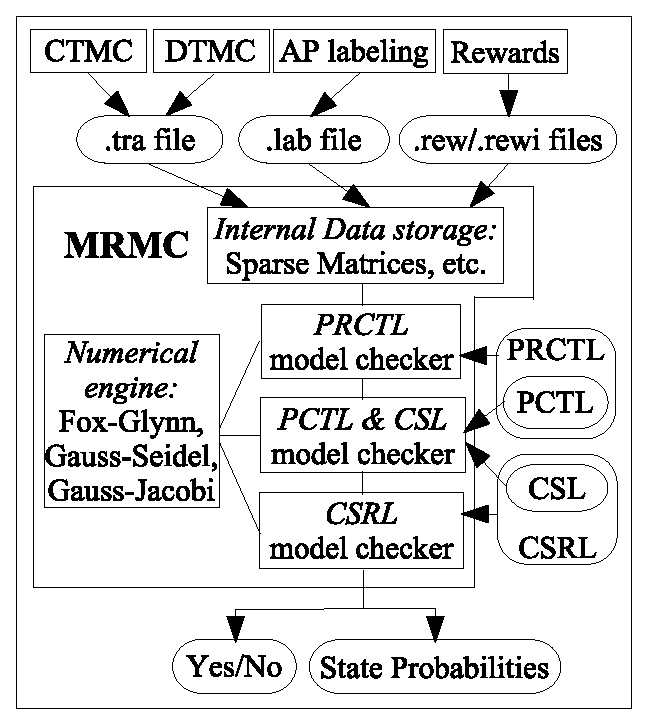
\includegraphics[scale=0.7, angle=0]{qest_05_figure_01.eps}
	\end{center}
	\caption{\emph{MRMC} inputs and outputs, tool structure \label{fig:general}}
\end{figure}

MRMC is a command-line tool, and expects four input files: a {\tt .tra}-file
describing the probability or rate matrix, a {\tt .lab}-file indicating the
state-labeling with atomic propositions, a {\tt .rew}-file specifying the
state reward structure, and a {\tt .rewi}-file specifying the
impulse reward structure.
For CSL and PCTL verification, the latter two files may be omitted.
A sketch of the tool architecture is provided in Fig.~\ref{fig:general}.

%------------------------------------------------------------------------- 
\Section{Outlook}

MRMC will further be used as an experimental platform for more advanced 
algorithms for checking time- and reward bounded properties and for
abstraction techniques.

\small{\bibliography{global_etmcc}}

\end{document}